
\section{Results}
\subsection{Original 4-bit mechanism benchmark}
Table~\ref{tab:mechanism} and Figure~\ref{fig:mechanism} summarize the mechanism benchmark. Compiling all 384 coordinates into 4-bit lookup tables matches the FP32 linear teacher within measurement noise, showing that the 4-bit substrate itself is not the principal bottleneck in this structured-label setting. Sparsifying to 28 unary terms plus four interactions retains 0.9015 mean F1, or 96.6\% of the teacher's F1. The largest gain comes from residual optimization, not interactions: boosted unary LUTs reach 0.8993, whereas independently estimated LLR factors reach 0.8152.

\begin{table}[t]
\centering
\caption{Mechanism benchmark (14 concepts).}
\label{tab:mechanism}
\small
\begin{tabular}{lcc}
\toprule
Method & Mean F1 & Mean AP\\
\midrule
FP32 linear & 0.9331 & 0.9596\\
Compiled linear, 384 LUTs & \textbf{0.9334} & \textbf{0.9596}\\
Boosted LUT + 4 pairs & 0.9015 & 0.9388\\
Boosted unary LUT & 0.8993 & 0.9372\\
Compiled linear, 28 coords & 0.8619 & 0.9102\\
LLR + EB + mRMR & 0.8346 & 0.8902\\
LLR factor & 0.8152 & 0.8724\\
\bottomrule
\end{tabular}
\end{table}

\begin{figure}[t]
\centering
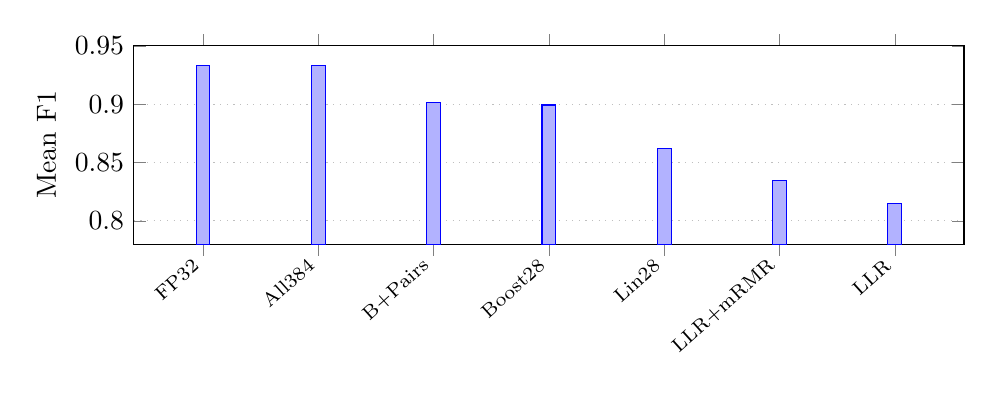
\begin{tikzpicture}
\begin{axis}[
  width=\columnwidth,height=4.1cm,
  ybar, ymin=0.78,ymax=0.95,
  ylabel={Mean F1},
  symbolic x coords={FP32,All384,B+Pairs,Boost28,Lin28,LLR+mRMR,LLR},
  xtick=data, x tick label style={rotate=42,anchor=east,font=\scriptsize},
  ymajorgrids=true, grid style={dotted},
  bar width=5pt,
]
\addplot coordinates {(FP32,0.9331) (All384,0.9334) (B+Pairs,0.9015) (Boost28,0.8993) (Lin28,0.8619) (LLR+mRMR,0.8346) (LLR,0.8152)};
\end{axis}
\end{tikzpicture}
\caption{Residual-optimized LUTs close most of the gap to the full-precision linear classifier in the original structured-label mechanism benchmark.}
\label{fig:mechanism}
\end{figure}

\paragraph{Ablations.} At a fixed 192-byte item budget, 384 four-bit coordinates outperform 768 two-bit coordinates (0.8993 vs. 0.8894 mean F1) and 1,536 one-bit random directions (0.8630). Power whitening consistently hurts: $\gamma=0.25,0.5,0.75,1.0$ produce 0.8944, 0.8654, 0.7993, and 0.6881 F1 respectively. Uniform and quantile 4-bit bins are effectively tied.

These ablations diagnose the original sparse-LUT compiler under structured labels; they should not be read as proving that four bits or random rotation are globally optimal. The independent-teacher benchmark below is the model-selection experiment. There, the full-run sparse ordering is RSA4 $>$ RSA2 $>$ RSA1, while the centered binary linear compiler provides a better compact Pareto point than any sparse \rsa variant.
